%%____________________________________________________________________________||
\section{Characterisation of the signal and control regions}
\label{sec:yields}

%%____________________________________________________________________________||
% \subsection{Key distributions for the hadronic signal
%   region\label{sec:mc-data-comp}}
%
% %Distributions of key analysis variables 
% The hadronic signal region selection is detailed in Sec.~\ref{sec:hadSelection}.

%%____________________________________________________________________________||
\subsection{Breakdown of SM backgrounds in the hadronic signal
  region\label{sec:bkgd-comp}}

In the absence of multijet events from QCD, the remaining significant
backgrounds in the signal region are expected to stem from SM
processes with genuine \met in the final state. For the low jet
multiplicity categories, the largest backgrounds with genuine \met are
generally from the associated production of W or Z bosons with jets,
followed by either the weak decays \znunu\ or \wtaunu, where the
$\tau$ decays hadronically and is identified as a jet, or by leptonic
decays that are outside acceptance or not rejected by the dedicated
electron or muon vetoes. For the higher jet multiplicity categories,
top quark production followed by semileptonic weak top quark decay
becomes important. The relative contribution from \ttbar is enhanced
or suppressed depending on the number of b-jets required. 
% A breakdown
% of the relative contributions of the SM backgrounds, as given by
% simulation, in the different (\njet, \nb, \scalht) bins can be found
% in Table~\ref{tab:backgrounds}. 
Plots showing the yields for these electroweak backgrounds can be seen in Table~\ref{tab:ewk-bkgd}.
A breakdown of the three
dominant channels, \ttbar, \zInv~ and W~+~jets, are shown in Tables \ref{tab:tt-bkgd}, 
\ref{tab:zinv-bkgd} and \ref{tab:wjet-bkgd} respectively for 3\ifb. The contribution from
other sources, such as the single top and diboson channels, was found to be
negligible so are not shown.

%\begin{landscape}
\begin{table}[h]
  \scriptsize
  \centering
  \topcaption{Electroweak background yields for each bin in the signal region for 3\ifb.
    The letter ``a'' in \njet \eg ``2a''  indicates the asymmetric \njet bins.
    \label{tab:ewk-bkgd}}
  \begin{tabular}
    {c|c|ccccccc}
    \hline\hline
          &     & \multicolumn{7}{c}{\scalht (\gev)} \\ 
    \njet & \nb & 200-250 & 250-300 & 300-350 & 350-400 & 400-600 & 600-800 & 800-$\infty$ \\ 
    \hline
	2 & 0 & 1399.45 $\pm$18.22 & 1462.74 $\pm$17.04 & 953.49 $\pm$12.91 & 571.77 $\pm$8.32 & 667.56 $\pm$4.87 & 80.60 $\pm$1.77 & 225.44 $\pm$2.07 \\ 
	2 & 1 & 165.32 $\pm$5.50 & 168.70 $\pm$5.43 & 111.48 $\pm$4.35 & 64.78 $\pm$2.96 & 75.64 $\pm$2.18 & 10.50 $\pm$1.61 & 28.62 $\pm$1.64 \\ 
	2 & 2 & 10.24 $\pm$1.87 & 13.91 $\pm$2.08 & 6.32 $\pm$1.75 & 3.99 $\pm$1.66 & 4.82 $\pm$1.61 & 0.62 $\pm$1.57 & 1.34 $\pm$1.58 \\ 
	3 & 0 & 2.42 $\pm$1.65 & 281.42 $\pm$7.49 & 790.41 $\pm$12.34 & 799.29 $\pm$10.25 & 1252.98 $\pm$7.57 & 166.87 $\pm$2.06 & 305.68 $\pm$2.27 \\ 
	3 & 1 & 0.45 $\pm$1.58 & 69.14 $\pm$3.54 & 161.42 $\pm$5.16 & 171.54 $\pm$4.79 & 251.75 $\pm$4.40 & 30.67 $\pm$1.85 & 60.33 $\pm$1.83 \\ 
	3 & 2 & 0.35 $\pm$1.59 & 10.92 $\pm$1.87 & 32.85 $\pm$2.47 & 38.34 $\pm$2.55 & 53.53 $\pm$2.57 & 4.87 $\pm$1.65 & 6.80 $\pm$1.63 \\ 
	3 & $\ge3$ & 0.00 $\pm$1.57 & 0.19 $\pm$1.58 & 1.54 $\pm$1.61 & 2.15 $\pm$1.62 & 2.93 $\pm$1.65 & 0.37 $\pm$1.58 & 0.15 $\pm$1.57 \\ 
	4 & 0 & - & 0.87 $\pm$1.59 & 122.30 $\pm$5.13 & 338.35 $\pm$7.26 & 1036.95 $\pm$8.07 & 194.92 $\pm$2.32 & 270.03 $\pm$2.42 \\ 
	4 & 1 & - & 0.57 $\pm$1.59 & 47.09 $\pm$2.96 & 137.16 $\pm$4.34 & 388.66 $\pm$5.96 & 59.21 $\pm$2.30 & 79.28 $\pm$2.31 \\ 
	4 & 2 & - & 0.29 $\pm$1.58 & 18.88 $\pm$2.23 & 61.13 $\pm$2.95 & 155.87 $\pm$4.15 & 17.69 $\pm$1.91 & 19.60 $\pm$1.89 \\ 
	4 & $\ge3$ & - & 0.00 $\pm$1.57 & 1.05 $\pm$1.59 & 5.50 $\pm$1.74 & 11.39 $\pm$1.86 & 1.93 $\pm$1.62 & 1.50 $\pm$1.60 \\ 
	$\ge5$ & 0 & - & - & 0.01 $\pm$1.57 & 18.42 $\pm$2.28 & 414.17 $\pm$5.61 & 187.27 $\pm$2.82 & 268.19 $\pm$2.75 \\ 
	$\ge5$ & 1 & - & - & 0.48 $\pm$1.58 & 10.94 $\pm$1.94 & 279.70 $\pm$5.27 & 109.96 $\pm$3.21 & 157.71 $\pm$3.60 \\ 
	$\ge5$ & 2 & - & - & 0.10 $\pm$1.58 & 4.88 $\pm$1.72 & 162.80 $\pm$4.16 & 62.16 $\pm$2.89 & 86.09 $\pm$3.24 \\ 
	$\ge5$ & $\ge3$ & - & - & 0.00 $\pm$1.57 & 0.76 $\pm$1.59 & 26.94 $\pm$2.26 & 12.23 $\pm$1.91 & 18.00 $\pm$1.99 \\ 
	2a & 0 & 7384.63 $\pm$44.69 & 2198.31 $\pm$20.57 & 828.51 $\pm$11.91 & 336.40 $\pm$6.44 & 272.33 $\pm$3.37 & 23.50 $\pm$1.63 & 26.38 $\pm$1.62 \\ 
	2a & 1 & 762.05 $\pm$12.53 & 223.71 $\pm$6.13 & 88.12 $\pm$3.98 & 32.70 $\pm$2.22 & 27.74 $\pm$1.77 & 2.35 $\pm$1.58 & 2.68 $\pm$1.58 \\ 
	2a & 2 & 51.57 $\pm$3.20 & 14.52 $\pm$2.04 & 5.14 $\pm$1.71 & 2.33 $\pm$1.62 & 1.51 $\pm$1.58 & 0.12 $\pm$1.57 & 0.17 $\pm$1.58 \\ 
	3a & 0 & 2123.67 $\pm$23.89 & 2052.57 $\pm$20.59 & 1063.87 $\pm$14.44 & 355.14 $\pm$6.96 & 182.25 $\pm$3.33 & 9.50 $\pm$1.60 & 11.95 $\pm$1.60 \\ 
	3a & 1 & 449.85 $\pm$9.12 & 466.24 $\pm$8.69 & 239.34 $\pm$6.26 & 76.98 $\pm$3.42 & 30.14 $\pm$1.92 & 1.25 $\pm$1.58 & 1.70 $\pm$1.58 \\ 
	3a & 2 & 85.98 $\pm$3.72 & 85.11 $\pm$3.59 & 50.56 $\pm$2.82 & 17.92 $\pm$2.07 & 4.70 $\pm$1.64 & 0.11 $\pm$1.57 & 0.03 $\pm$1.58 \\ 
	3a & $\ge3$ & 3.10 $\pm$1.65 & 2.98 $\pm$1.65 & 2.13 $\pm$1.62 & 0.83 $\pm$1.59 & 0.16 $\pm$1.58 & 0.00 $\pm$1.57 & 0.00 $\pm$1.57 \\ 
	4a & 0 & - & 225.40 $\pm$6.81 & 638.08 $\pm$11.53 & 429.52 $\pm$8.47 & 276.02 $\pm$4.65 & 5.13 $\pm$1.59 & 4.56 $\pm$1.58 \\ 
	4a & 1 & - & 80.18 $\pm$3.71 & 264.11 $\pm$6.31 & 176.44 $\pm$5.04 & 95.93 $\pm$3.34 & 1.14 $\pm$1.58 & 0.92 $\pm$1.58 \\ 
	4a & 2 & - & 23.55 $\pm$2.17 & 100.16 $\pm$3.71 & 68.38 $\pm$3.17 & 38.55 $\pm$2.50 & 0.26 $\pm$1.58 & 0.10 $\pm$1.57 \\ 
	4a & $\ge3$ & - & 2.40 $\pm$1.64 & 8.47 $\pm$1.81 & 5.70 $\pm$1.73 & 3.09 $\pm$1.65 & 0.10 $\pm$1.58 & 0.01 $\pm$1.57 \\ 
	$\ge5$a & 0 & - & - & 58.29 $\pm$3.66 & 165.26 $\pm$5.66 & 261.03 $\pm$5.38 & 9.78 $\pm$1.66 & 2.37 $\pm$1.59 \\ 
	$\ge5$a & 1 & - & - & 34.28 $\pm$2.56 & 109.71 $\pm$4.01 & 198.81 $\pm$4.64 & 5.51 $\pm$1.71 & 1.05 $\pm$1.59 \\ 
	$\ge5$a & 2 & - & - & 18.21 $\pm$2.05 & 60.50 $\pm$2.94 & 116.74 $\pm$3.75 & 4.23 $\pm$1.68 & 0.27 $\pm$1.58 \\ 
	$\ge5$a & $\ge3$ & - & - & 2.49 $\pm$1.64 & 8.36 $\pm$1.83 & 18.60 $\pm$2.05 & 0.79 $\pm$1.59 & 0.01 $\pm$1.57 \\ 
\hline\hline
  \end{tabular}
\end{table}

\newpage
\begin{table}[h]
  \scriptsize
  \centering
  \topcaption{\ttbar background yields for each bin in the signal region for 3\ifb.
    The letter ``a'' in \njet \eg ``2a''  indicates the asymmetric \njet bins.
    \label{tab:tt-bkgd}}
  \begin{tabular}
    {c|c|ccccccc}
    \hline\hline
          &     & \multicolumn{7}{c}{\scalht (\gev)} \\ 
    \njet & \nb & 200-250 & 250-300 & 300-350 & 350-400 & 400-600 & 600-800 & 800-$\infty$ \\  
    \hline
	2 & 0 & 43.69 $\pm$2.04 & 38.44 $\pm$1.91 & 14.69 $\pm$1.18 & 6.20 $\pm$0.77 & 4.29 $\pm$0.64 & 0.10 $\pm$0.13 & 0.76 $\pm$0.27 \\ 
	2 & 1 & 47.31 $\pm$2.12 & 38.06 $\pm$1.91 & 16.60 $\pm$1.26 & 6.77 $\pm$0.80 & 3.43 $\pm$0.57 & 0.57 $\pm$0.23 & 0.19 $\pm$0.15 \\ 
	2 & 2 & 3.53 $\pm$0.58 & 2.67 $\pm$0.50 & 0.67 $\pm$0.25 & 0.95 $\pm$0.30 & 0.48 $\pm$0.21 & 0.00 $\pm$0.11 & 0.10 $\pm$0.13 \\ 
	3 & 0 & 0.19 $\pm$0.15 & 21.94 $\pm$1.45 & 45.50 $\pm$2.08 & 36.34 $\pm$1.86 & 41.21 $\pm$1.98 & 1.62 $\pm$0.39 & 2.67 $\pm$0.50 \\ 
	3 & 1 & 0.10 $\pm$0.13 & 33.39 $\pm$1.78 & 71.25 $\pm$2.61 & 62.76 $\pm$2.45 & 66.58 $\pm$2.52 & 3.05 $\pm$0.54 & 3.82 $\pm$0.60 \\ 
	3 & 2 & 0.00 $\pm$0.11 & 6.87 $\pm$0.81 & 20.99 $\pm$1.41 & 24.32 $\pm$1.52 & 31.38 $\pm$1.73 & 2.19 $\pm$0.46 & 1.53 $\pm$0.38 \\ 
	3 & $\ge3$ & 0.00 $\pm$0.11 & 0.10 $\pm$0.13 & 1.05 $\pm$0.32 & 1.53 $\pm$0.38 & 2.48 $\pm$0.49 & 0.29 $\pm$0.17 & 0.00 $\pm$0.11 \\ 
	4 & 0 & - & 0.19 $\pm$0.15 & 13.83 $\pm$1.15 & 40.63 $\pm$1.97 & 85.85 $\pm$2.86 & 7.92 $\pm$0.87 & 7.73 $\pm$0.86 \\ 
	4 & 1 & - & 0.57 $\pm$0.23 & 29.28 $\pm$1.67 & 81.56 $\pm$2.79 & 205.94 $\pm$4.43 & 18.70 $\pm$1.34 & 17.84 $\pm$1.30 \\ 
	4 & 2 & - & 0.29 $\pm$0.17 & 14.78 $\pm$1.19 & 49.79 $\pm$2.18 & 117.80 $\pm$3.35 & 10.78 $\pm$1.01 & 9.92 $\pm$0.97 \\ 
	4 & $\ge3$ & - & 0.00 $\pm$0.11 & 0.67 $\pm$0.25 & 4.20 $\pm$0.63 & 10.11 $\pm$0.98 & 1.43 $\pm$0.37 & 0.86 $\pm$0.29 \\ 
	$\ge5$ & 0 & - & - & 0.00 $\pm$0.11 & 4.10 $\pm$0.63 & 80.12 $\pm$2.76 & 25.47 $\pm$1.56 & 29.28 $\pm$1.67 \\ 
	$\ge5$ & 1 & - & - & 0.48 $\pm$0.21 & 8.39 $\pm$0.89 & 195.07 $\pm$4.31 & 67.15 $\pm$2.53 & 81.27 $\pm$2.78 \\ 
	$\ge5$ & 2 & - & - & 0.10 $\pm$0.13 & 4.86 $\pm$0.68 & 142.41 $\pm$3.69 & 51.22 $\pm$2.21 & 65.24 $\pm$2.49 \\ 
	$\ge5$ & $\ge3$ & - & - & 0.00 $\pm$0.11 & 0.76 $\pm$0.27 & 22.89 $\pm$1.48 & 11.35 $\pm$1.04 & 15.07 $\pm$1.20 \\ 
	2a & 0 & 204.89 $\pm$4.42 & 42.73 $\pm$2.02 & 9.63 $\pm$0.96 & 2.86 $\pm$0.52 & 0.86 $\pm$0.29 & 0.00 $\pm$0.11 & 0.00 $\pm$0.11 \\ 
	2a & 1 & 177.04 $\pm$4.11 & 39.49 $\pm$1.94 & 9.44 $\pm$0.95 & 2.10 $\pm$0.45 & 1.05 $\pm$0.32 & 0.00 $\pm$0.11 & 0.00 $\pm$0.11 \\ 
	2a & 2 & 11.45 $\pm$1.04 & 2.38 $\pm$0.48 & 0.67 $\pm$0.25 & 0.29 $\pm$0.17 & 0.10 $\pm$0.13 & 0.00 $\pm$0.11 & 0.10 $\pm$0.13 \\ 
	3a & 0 & 153.00 $\pm$3.82 & 143.84 $\pm$3.70 & 59.24 $\pm$2.38 & 14.98 $\pm$1.20 & 3.53 $\pm$0.58 & 0.10 $\pm$0.13 & 0.19 $\pm$0.15 \\ 
	3a & 1 & 209.95 $\pm$4.48 & 214.72 $\pm$4.53 & 105.97 $\pm$3.18 & 28.52 $\pm$1.65 & 5.44 $\pm$0.72 & 0.00 $\pm$0.11 & 0.00 $\pm$0.11 \\ 
	3a & 2 & 52.75 $\pm$2.24 & 53.70 $\pm$2.26 & 33.29 $\pm$1.78 & 10.97 $\pm$1.02 & 1.72 $\pm$0.40 & 0.00 $\pm$0.11 & 0.10 $\pm$0.13 \\ 
	3a & $\ge3$ & 2.29 $\pm$0.47 & 2.10 $\pm$0.45 & 1.43 $\pm$0.37 & 0.76 $\pm$0.27 & 0.10 $\pm$0.13 & 0.00 $\pm$0.11 & 0.00 $\pm$0.11 \\ 
	4a & 0 & - & 27.19 $\pm$1.61 & 80.51 $\pm$2.77 & 46.83 $\pm$2.11 & 22.99 $\pm$1.48 & 0.00 $\pm$0.11 & 0.00 $\pm$0.11 \\ 
	4a & 1 & - & 45.98 $\pm$2.09 & 162.44 $\pm$3.94 & 102.35 $\pm$3.12 & 48.17 $\pm$2.14 & 0.19 $\pm$0.15 & 0.10 $\pm$0.13 \\ 
	4a & 2 & - & 19.84 $\pm$1.38 & 81.75 $\pm$2.79 & 54.18 $\pm$2.27 & 29.09 $\pm$1.67 & 0.00 $\pm$0.11 & 0.00 $\pm$0.11 \\ 
	4a & $\ge3$ & - & 1.72 $\pm$0.40 & 7.25 $\pm$0.83 & 5.34 $\pm$0.71 & 2.48 $\pm$0.49 & 0.10 $\pm$0.13 & 0.00 $\pm$0.11 \\ 
	$\ge5$a & 0 & - & - & 13.64 $\pm$1.14 & 37.39 $\pm$1.89 & 56.85 $\pm$2.33 & 1.81 $\pm$0.42 & 0.48 $\pm$0.21 \\ 
	$\ge5$a & 1 & - & - & 23.85 $\pm$1.51 & 82.51 $\pm$2.81 & 152.14 $\pm$3.81 & 3.34 $\pm$0.56 & 0.57 $\pm$0.23 \\ 
	$\ge5$a & 2 & - & - & 16.02 $\pm$1.24 & 55.32 $\pm$2.30 & 103.69 $\pm$3.14 & 3.72 $\pm$0.60 & 0.19 $\pm$0.15 \\ 
	$\ge5$a & $\ge3$ & - & - & 2.19 $\pm$0.46 & 8.30 $\pm$0.89 & 16.69 $\pm$1.26 & 0.76 $\pm$0.27 & 0.00 $\pm$0.11 \\ 
\hline\hline
  \end{tabular}
\end{table}

\newpage
\begin{table}[h]
  \scriptsize
  \centering
  \topcaption{W~+~jets background yields for each bin in the signal region for 3\ifb.
    The letter ``a'' in \njet \eg ``2a''  indicates the asymmetric \njet bins.
    \label{tab:wjet-bkgd}}
  \begin{tabular}
    {c|c|ccccccc}
    \hline\hline
          &     & \multicolumn{7}{c}{\scalht (\gev)} \\ 
    \njet & \nb & 200-250 & 250-300 & 300-350 & 350-400 & 400-600 & 600-800 & 800-$\infty$ \\  
    \hline
	2 & 0 & 595.75 $\pm$15.92 & 589.10 $\pm$14.63 & 366.81 $\pm$10.99 & 217.75 $\pm$7.09 & 230.29 $\pm$4.12 & 21.13 $\pm$1.64 & 76.44 $\pm$1.86 \\ 
	2 & 1 & 44.42 $\pm$4.26 & 45.00 $\pm$4.22 & 33.60 $\pm$3.54 & 18.66 $\pm$2.45 & 22.02 $\pm$1.87 & 2.36 $\pm$1.53 & 9.12 $\pm$1.57 \\ 
	2 & 2 & 1.06 $\pm$1.59 & 3.17 $\pm$1.81 & 1.28 $\pm$1.59 & 1.06 $\pm$1.57 & 0.71 $\pm$1.53 & 0.09 $\pm$1.52 & 0.41 $\pm$1.52 \\ 
	3 & 0 & 0.71 $\pm$1.56 & 108.45 $\pm$6.38 & 342.08 $\pm$10.71 & 333.22 $\pm$8.78 & 491.72 $\pm$6.25 & 53.34 $\pm$1.81 & 110.50 $\pm$2.00 \\ 
	3 & 1 & 0.00 $\pm$1.52 & 13.88 $\pm$2.65 & 35.18 $\pm$3.64 & 43.00 $\pm$3.37 & 65.68 $\pm$2.60 & 7.91 $\pm$1.57 & 20.96 $\pm$1.62 \\ 
	3 & 2 & 0.35 $\pm$1.54 & 0.75 $\pm$1.56 & 3.44 $\pm$1.81 & 4.15 $\pm$1.72 & 5.61 $\pm$1.61 & 0.57 $\pm$1.52 & 1.33 $\pm$1.53 \\ 
	3 & $\ge3$ & 0.00 $\pm$1.52 & 0.00 $\pm$1.52 & 0.00 $\pm$1.52 & 0.02 $\pm$1.52 & 0.15 $\pm$1.52 & 0.02 $\pm$1.52 & 0.05 $\pm$1.52 \\ 
	4 & 0 & - & 0.00 $\pm$1.52 & 53.82 $\pm$4.50 & 143.21 $\pm$6.25 & 432.82 $\pm$6.64 & 65.53 $\pm$1.90 & 102.96 $\pm$1.97 \\ 
	4 & 1 & - & 0.00 $\pm$1.52 & 8.86 $\pm$2.27 & 21.81 $\pm$2.69 & 69.19 $\pm$2.77 & 14.30 $\pm$1.61 & 22.42 $\pm$1.63 \\ 
	4 & 2 & - & 0.00 $\pm$1.52 & 2.02 $\pm$1.82 & 3.88 $\pm$1.75 & 9.65 $\pm$1.73 & 1.78 $\pm$1.53 & 3.14 $\pm$1.54 \\ 
	4 & $\ge3$ & - & 0.00 $\pm$1.52 & 0.00 $\pm$1.52 & 0.71 $\pm$1.56 & 0.37 $\pm$1.53 & 0.09 $\pm$1.52 & 0.18 $\pm$1.52 \\ 
	$\ge5$ & 0 & - & - & 0.00 $\pm$1.52 & 7.32 $\pm$2.05 & 162.75 $\pm$4.47 & 66.85 $\pm$2.04 & 104.10 $\pm$2.01 \\ 
	$\ge5$ & 1 & - & - & 0.00 $\pm$1.52 & 2.07 $\pm$1.63 & 36.28 $\pm$2.53 & 16.08 $\pm$1.64 & 31.02 $\pm$1.67 \\ 
	$\ge5$ & 2 & - & - & 0.00 $\pm$1.52 & 0.13 $\pm$1.52 & 6.66 $\pm$1.69 & 2.94 $\pm$1.54 & 6.03 $\pm$1.55 \\ 
	$\ge5$ & $\ge3$ & - & - & 0.00 $\pm$1.52 & 0.00 $\pm$1.52 & 0.75 $\pm$1.55 & 0.41 $\pm$1.52 & 0.83 $\pm$1.53 \\ 
	2a & 0 & 3185.31 $\pm$39.22 & 855.15 $\pm$17.48 & 298.73 $\pm$10.01 & 111.65 $\pm$5.38 & 75.96 $\pm$2.83 & 5.11 $\pm$1.55 & 5.06 $\pm$1.55 \\ 
	2a & 1 & 215.63 $\pm$10.03 & 58.57 $\pm$4.75 & 26.76 $\pm$3.27 & 8.08 $\pm$1.87 & 6.47 $\pm$1.61 & 0.62 $\pm$1.52 & 0.65 $\pm$1.52 \\ 
	2a & 2 & 12.08 $\pm$2.53 & 2.53 $\pm$1.73 & 1.23 $\pm$1.59 & 0.53 $\pm$1.54 & 0.24 $\pm$1.52 & 0.02 $\pm$1.52 & 0.02 $\pm$1.52 \\ 
	3a & 0 & 911.15 $\pm$21.08 & 860.76 $\pm$17.78 & 439.76 $\pm$12.45 & 136.00 $\pm$5.93 & 57.60 $\pm$2.89 & 2.25 $\pm$1.53 & 2.51 $\pm$1.53 \\ 
	3a & 1 & 95.81 $\pm$6.66 & 99.33 $\pm$6.14 & 48.06 $\pm$4.28 & 17.52 $\pm$2.46 & 6.64 $\pm$1.64 & 0.33 $\pm$1.52 & 0.44 $\pm$1.52 \\ 
	3a & 2 & 11.50 $\pm$2.57 & 10.44 $\pm$2.40 & 4.58 $\pm$1.91 & 2.12 $\pm$1.66 & 0.57 $\pm$1.53 & 0.00 $\pm$1.52 & 0.00 $\pm$1.52 \\ 
	3a & $\ge3$ & 0.00 $\pm$1.52 & 0.00 $\pm$1.52 & 0.00 $\pm$1.52 & 0.04 $\pm$1.52 & 0.00 $\pm$1.52 & 0.00 $\pm$1.52 & 0.00 $\pm$1.52 \\ 
	4a & 0 & - & 88.53 $\pm$5.80 & 273.90 $\pm$10.01 & 186.05 $\pm$7.31 & 108.32 $\pm$3.88 & 1.27 $\pm$1.53 & 1.17 $\pm$1.53 \\ 
	4a & 1 & - & 14.19 $\pm$2.67 & 42.49 $\pm$4.07 & 30.80 $\pm$3.24 & 17.80 $\pm$2.03 & 0.21 $\pm$1.52 & 0.17 $\pm$1.52 \\ 
	4a & 2 & - & 0.71 $\pm$1.56 & 5.42 $\pm$2.00 & 4.59 $\pm$1.82 & 2.21 $\pm$1.57 & 0.05 $\pm$1.52 & 0.03 $\pm$1.52 \\ 
	4a & $\ge3$ & - & 0.00 $\pm$1.52 & 0.04 $\pm$1.52 & 0.09 $\pm$1.52 & 0.15 $\pm$1.52 & 0.00 $\pm$1.52 & 0.00 $\pm$1.52 \\ 
	$\ge5$a & 0 & - & - & 23.40 $\pm$3.18 & 68.79 $\pm$4.89 & 101.78 $\pm$4.40 & 3.16 $\pm$1.55 & 0.42 $\pm$1.52 \\ 
	$\ge5$a & 1 & - & - & 4.01 $\pm$1.88 & 13.14 $\pm$2.47 & 20.63 $\pm$2.24 & 0.94 $\pm$1.53 & 0.15 $\pm$1.52 \\ 
	$\ge5$a & 2 & - & - & 0.71 $\pm$1.56 & 1.72 $\pm$1.63 & 3.43 $\pm$1.65 & 0.09 $\pm$1.52 & 0.03 $\pm$1.52 \\ 
	$\ge5$a & $\ge3$ & - & - & 0.00 $\pm$1.52 & 0.02 $\pm$1.52 & 0.71 $\pm$1.55 & 0.00 $\pm$1.52 & 0.00 $\pm$1.52 \\ 
	
\hline\hline
  \end{tabular}
\end{table}

\newpage
\begin{table}[h]
  \scriptsize
  \centering
  \topcaption{\zInv~ background yields for each bin in the signal region for 3\ifb.
    The letter ``a'' in \njet \eg ``2a''  indicates the asymmetric \njet bins.}
  \label{tab:zinv-bkgd}
  \begin{tabular}
    {c|c|ccccccc}
    \hline\hline
          &     & \multicolumn{7}{c}{\scalht (\gev)} \\ 
    \njet & \nb & 200-250 & 250-300 & 300-350 & 350-400 & 400-600 & 600-800 & 800-$\infty$ \\  
    \hline
	2 & 0 & 749.19 $\pm$8.44 & 827.63 $\pm$8.37 & 568.18 $\pm$6.60 & 344.68 $\pm$4.15 & 431.15 $\pm$2.44 & 59.59 $\pm$0.59 & 148.31 $\pm$0.80 \\ 
	2 & 1 & 65.73 $\pm$2.48 & 80.67 $\pm$2.64 & 59.27 $\pm$2.12 & 37.60 $\pm$1.36 & 48.53 $\pm$0.84 & 7.20 $\pm$0.38 & 19.07 $\pm$0.43 \\ 
	2 & 2 & 5.21 $\pm$0.75 & 7.52 $\pm$0.87 & 4.51 $\pm$0.65 & 1.98 $\pm$0.41 & 3.30 $\pm$0.40 & 0.53 $\pm$0.34 & 0.73 $\pm$0.35 \\ 
	3 & 0 & 1.52 $\pm$0.49 & 147.44 $\pm$3.54 & 396.21 $\pm$5.55 & 426.78 $\pm$4.62 & 710.84 $\pm$3.21 & 111.62 $\pm$0.75 & 191.75 $\pm$0.89 \\ 
	3 & 1 & 0.17 $\pm$0.35 & 18.31 $\pm$1.28 & 47.44 $\pm$1.92 & 59.08 $\pm$1.66 & 107.89 $\pm$1.26 & 18.38 $\pm$0.43 & 34.53 $\pm$0.49 \\ 
	3 & 2 & 0.00 $\pm$0.34 & 2.60 $\pm$0.57 & 7.24 $\pm$0.81 & 8.27 $\pm$0.70 & 13.05 $\pm$0.52 & 2.07 $\pm$0.35 & 3.20 $\pm$0.36 \\ 
	3 & $\ge3$ & 0.00 $\pm$0.34 & 0.09 $\pm$0.35 & 0.38 $\pm$0.37 & 0.28 $\pm$0.35 & 0.46 $\pm$0.35 & 0.07 $\pm$0.34 & 0.10 $\pm$0.34 \\ 
	4 & 0 & - & 0.68 $\pm$0.40 & 52.66 $\pm$2.08 & 151.49 $\pm$2.96 & 512.02 $\pm$2.96 & 121.48 $\pm$0.80 & 157.82 $\pm$0.82 \\ 
	4 & 1 & - & 0.00 $\pm$0.34 & 8.43 $\pm$0.86 & 27.56 $\pm$1.27 & 98.08 $\pm$1.28 & 24.78 $\pm$0.47 & 36.24 $\pm$0.49 \\ 
	4 & 2 & - & 0.00 $\pm$0.34 & 1.21 $\pm$0.44 & 5.02 $\pm$0.63 & 18.20 $\pm$0.64 & 4.24 $\pm$0.37 & 5.30 $\pm$0.37 \\ 
	4 & $\ge3$ & - & 0.00 $\pm$0.34 & 0.09 $\pm$0.35 & 0.28 $\pm$0.35 & 1.04 $\pm$0.36 & 0.30 $\pm$0.34 & 0.35 $\pm$0.34 \\ 
	$\ge5$ & 0 & - & - & 0.01 $\pm$0.34 & 6.87 $\pm$0.73 & 167.14 $\pm$1.82 & 94.88 $\pm$0.82 & 133.80 $\pm$0.77 \\ 
	$\ge5$ & 1 & - & - & 0.00 $\pm$0.34 & 1.03 $\pm$0.40 & 39.31 $\pm$0.94 & 24.31 $\pm$0.49 & 40.50 $\pm$0.51 \\ 
	$\ge5$ & 2 & - & - & 0.00 $\pm$0.34 & 0.11 $\pm$0.34 & 9.10 $\pm$0.57 & 5.29 $\pm$0.38 & 9.03 $\pm$0.39 \\ 
	$\ge5$ & $\ge3$ & - & - & 0.00 $\pm$0.34 & 0.00 $\pm$0.34 & 0.94 $\pm$0.36 & 0.63 $\pm$0.35 & 1.21 $\pm$0.35 \\ 
	2a & 0 & 3951.84 $\pm$20.57 & 1287.73 $\pm$10.42 & 518.47 $\pm$6.36 & 220.70 $\pm$3.43 & 195.66 $\pm$1.76 & 18.21 $\pm$0.44 & 21.32 $\pm$0.44 \\ 
	2a & 1 & 347.76 $\pm$5.94 & 119.87 $\pm$3.18 & 50.76 $\pm$1.99 & 21.84 $\pm$1.08 & 20.14 $\pm$0.63 & 1.73 $\pm$0.35 & 2.11 $\pm$0.35 \\ 
	2a & 2 & 26.98 $\pm$1.63 & 9.36 $\pm$0.94 & 2.87 $\pm$0.55 & 1.30 $\pm$0.40 & 1.07 $\pm$0.36 & 0.10 $\pm$0.34 & 0.06 $\pm$0.34 \\ 
	3a & 0 & 1046.96 $\pm$10.51 & 1034.67 $\pm$9.46 & 557.97 $\pm$6.65 & 200.33 $\pm$3.28 & 119.78 $\pm$1.48 & 7.00 $\pm$0.38 & 9.25 $\pm$0.39 \\ 
	3a & 1 & 122.53 $\pm$3.56 & 127.65 $\pm$3.30 & 73.86 $\pm$2.41 & 26.75 $\pm$1.19 & 17.45 $\pm$0.63 & 0.92 $\pm$0.35 & 1.26 $\pm$0.35 \\ 
	3a & 2 & 16.77 $\pm$1.28 & 17.29 $\pm$1.26 & 10.26 $\pm$0.94 & 3.49 $\pm$0.51 & 2.14 $\pm$0.37 & 0.11 $\pm$0.34 & 0.12 $\pm$0.34 \\ 
	3a & $\ge3$ & 0.59 $\pm$0.39 & 0.77 $\pm$0.41 & 0.43 $\pm$0.37 & 0.02 $\pm$0.34 & 0.07 $\pm$0.34 & 0.00 $\pm$0.34 & 0.00 $\pm$0.34 \\ 
	4a & 0 & - & 107.08 $\pm$3.07 & 281.21 $\pm$4.78 & 194.63 $\pm$3.48 & 142.82 $\pm$1.76 & 3.76 $\pm$0.37 & 3.39 $\pm$0.36 \\ 
	4a & 1 & - & 16.00 $\pm$1.21 & 47.78 $\pm$1.97 & 34.89 $\pm$1.47 & 26.06 $\pm$0.81 & 0.74 $\pm$0.35 & 0.66 $\pm$0.35 \\ 
	4a & 2 & - & 2.48 $\pm$0.56 & 8.25 $\pm$0.87 & 7.04 $\pm$0.72 & 4.75 $\pm$0.43 & 0.10 $\pm$0.34 & 0.07 $\pm$0.34 \\ 
	4a & $\ge3$ & - & 0.25 $\pm$0.36 & 0.67 $\pm$0.40 & 0.51 $\pm$0.36 & 0.30 $\pm$0.35 & 0.01 $\pm$0.34 & 0.01 $\pm$0.34 \\ 
	$\ge5$a & 0 & - & - & 20.38 $\pm$1.33 & 56.52 $\pm$1.99 & 99.75 $\pm$1.85 & 4.83 $\pm$0.38 & 1.46 $\pm$0.35 \\ 
	$\ge5$a & 1 & - & - & 4.41 $\pm$0.68 & 11.43 $\pm$0.93 & 20.96 $\pm$0.85 & 1.25 $\pm$0.35 & 0.32 $\pm$0.34 \\ 
	$\ge5$a & 2 & - & - & 0.99 $\pm$0.43 & 3.17 $\pm$0.58 & 4.73 $\pm$0.49 & 0.29 $\pm$0.34 & 0.05 $\pm$0.34 \\ 
	$\ge5$a & $\ge3$ & - & - & 0.19 $\pm$0.35 & 0.13 $\pm$0.35 & 0.42 $\pm$0.35 & 0.02 $\pm$0.34 & 0.01 $\pm$0.34 \\ 
	
\hline\hline
  \end{tabular}
\end{table}

%%____________________________________________________________________________||
\newpage
\subsection{Yields in the control samples}

The yields in the \mj, \mmj, \ej, \eej and \gj control samples can be seen in
Tables~\ref{tab:mj-bkgd}, \ref{tab:ej-bkgd}, \ref{tab:mmj-bkgd}, \ref{tab:eej-bkgd}
and \ref{tab:gj-bkgd} respectively or 3 \ifb. 
The number of events in each of these bins is important for
working out how far we can extend in our analysis bins. We require there to be
enough events in the control samples to allow robust data driven prediction of
the backgrounds.

\begin{table}[h]
  \scriptsize
  \centering
  \topcaption{Yields in the \mj control region for 3\ifb.
  The letter ``a'' in \njet \eg ``2a''  indicates the asymmetric \njet bins.}
  \label{tab:mj-bkgd}
  \begin{tabular}
    {c|c|ccccccc}
    \hline\hline
          &     & \multicolumn{7}{c}{\scalht (\gev)} \\ 
    \njet & \nb & 200-250 & 250-300 & 300-350 & 350-400 & 400-600 & 600-800 & 800-$\infty$ \\  
    \hline
	2 & 0 & 4346.17 $\pm$41.15 & 5108.20 $\pm$42.07 & 3484.16 $\pm$33.25 & 2168.42 $\pm$21.37 & 3249.40 $\pm$14.21 & 709.92 $\pm$4.30 & 334.45 $\pm$2.93 \\ 
	2 & 1 & 822.03 $\pm$15.39 & 936.70 $\pm$16.11 & 596.16 $\pm$12.74 & 353.38 $\pm$8.76 & 518.38 $\pm$7.79 & 114.24 $\pm$3.29 & 50.16 $\pm$2.16 \\ 
	2 & 2 & 167.05 $\pm$5.07 & 159.78 $\pm$5.24 & 84.70 $\pm$3.84 & 47.65 $\pm$2.99 & 54.87 $\pm$3.00 & 10.96 $\pm$1.79 & 3.51 $\pm$1.60 \\ 
	3 & 0 & 13.13 $\pm$2.48 & 1320.72 $\pm$20.72 & 2448.70 $\pm$26.68 & 2081.66 $\pm$20.02 & 3798.46 $\pm$16.08 & 951.99 $\pm$5.34 & 486.15 $\pm$3.81 \\ 
	3 & 1 & 10.62 $\pm$1.98 & 700.01 $\pm$11.33 & 1242.86 $\pm$14.83 & 1021.16 $\pm$12.52 & 1537.12 $\pm$13.74 & 313.53 $\pm$5.78 & 139.21 $\pm$3.66 \\ 
	3 & 2 & 3.75 $\pm$1.66 & 315.92 $\pm$6.47 & 559.56 $\pm$8.33 & 420.24 $\pm$7.17 & 575.91 $\pm$8.25 & 97.94 $\pm$3.62 & 34.68 $\pm$2.34 \\ 
	3 & $\ge3$ & 0.29 $\pm$1.54 & 16.22 $\pm$1.99 & 30.11 $\pm$2.33 & 22.34 $\pm$2.13 & 32.39 $\pm$2.38 & 6.61 $\pm$1.74 & 1.72 $\pm$1.58 \\ 
	4 & 0 & - & 6.86 $\pm$2.05 & 318.04 $\pm$9.19 & 827.83 $\pm$12.86 & 2535.78 $\pm$14.67 & 806.62 $\pm$5.86 & 441.39 $\pm$3.97 \\ 
	4 & 1 & - & 5.53 $\pm$1.71 & 319.27 $\pm$6.82 & 803.91 $\pm$10.12 & 2162.45 $\pm$15.65 & 533.13 $\pm$7.62 & 234.44 $\pm$4.85 \\ 
	4 & 2 & - & 2.79 $\pm$1.61 & 192.62 $\pm$4.86 & 515.10 $\pm$7.69 & 1342.57 $\pm$12.29 & 282.97 $\pm$5.80 & 99.48 $\pm$3.73 \\ 
	4 & $\ge3$ & - & 0.48 $\pm$1.55 & 16.00 $\pm$1.97 & 47.48 $\pm$2.71 & 129.33 $\pm$4.00 & 29.24 $\pm$2.26 & 12.44 $\pm$1.89 \\ 
	$\ge5$ & 0 & - & - & 0.92 $\pm$1.57 & 57.26 $\pm$3.45 & 1069.76 $\pm$9.99 & 697.24 $\pm$6.78 & 505.51 $\pm$5.13 \\ 
	$\ge5$ & 1 & - & - & 1.53 $\pm$1.58 & 89.98 $\pm$3.50 & 1708.74 $\pm$13.45 & 1014.89 $\pm$10.21 & 651.84 $\pm$8.02 \\ 
	$\ge5$ & 2 & - & - & 1.34 $\pm$1.57 & 64.64 $\pm$2.92 & 1274.98 $\pm$11.54 & 800.16 $\pm$9.24 & 488.96 $\pm$7.26 \\ 
	$\ge5$ & $\ge3$ & - & - & 0.10 $\pm$1.54 & 8.67 $\pm$1.77 & 196.88 $\pm$4.67 & 155.19 $\pm$4.23 & 112.46 $\pm$3.70 \\ 
	2a & 0 & 18335.54 $\pm$90.97 & 5687.87 $\pm$44.73 & 2099.10 $\pm$25.98 & 905.73 $\pm$14.33 & 807.85 $\pm$7.62 & 91.87 $\pm$2.09 & 22.38 $\pm$1.65 \\ 
	2a & 1 & 3097.49 $\pm$31.18 & 862.02 $\pm$15.71 & 295.56 $\pm$9.27 & 124.27 $\pm$5.34 & 112.53 $\pm$3.79 & 12.60 $\pm$1.72 & 3.22 $\pm$1.58 \\ 
	2a & 2 & 447.75 $\pm$8.40 & 97.08 $\pm$4.42 & 25.10 $\pm$2.58 & 11.22 $\pm$1.99 & 11.36 $\pm$1.88 & 0.99 $\pm$1.55 & 0.50 $\pm$1.54 \\ 
	3a & 0 & 6664.32 $\pm$52.07 & 6233.59 $\pm$45.32 & 2428.40 $\pm$27.14 & 908.41 $\pm$13.99 & 665.09 $\pm$7.72 & 56.30 $\pm$1.93 & 11.73 $\pm$1.61 \\ 
	3a & 1 & 2986.57 $\pm$24.21 & 3057.86 $\pm$23.85 & 1005.44 $\pm$14.02 & 307.04 $\pm$7.44 & 210.20 $\pm$5.31 & 16.21 $\pm$1.92 & 2.60 $\pm$1.58 \\ 
	3a & 2 & 1140.59 $\pm$12.14 & 1210.02 $\pm$12.31 & 361.00 $\pm$7.09 & 94.94 $\pm$3.82 & 54.24 $\pm$2.96 & 3.02 $\pm$1.62 & 0.57 $\pm$1.55 \\ 
	3a & $\ge3$ & 57.36 $\pm$2.89 & 66.18 $\pm$3.05 & 19.53 $\pm$2.07 & 2.83 $\pm$1.63 & 0.91 $\pm$1.58 & 0.22 $\pm$1.54 & 0.11 $\pm$1.54 \\ 
	4a & 0 & - & 1143.62 $\pm$18.96 & 1646.08 $\pm$21.29 & 833.98 $\pm$13.19 & 551.06 $\pm$7.52 & 30.48 $\pm$1.89 & 4.60 $\pm$1.57 \\ 
	4a & 1 & - & 1014.91 $\pm$12.19 & 1588.03 $\pm$14.97 & 770.43 $\pm$10.26 & 386.17 $\pm$6.96 & 15.49 $\pm$1.94 & 1.94 $\pm$1.56 \\ 
	4a & 2 & - & 556.68 $\pm$8.10 & 952.00 $\pm$10.48 & 442.91 $\pm$7.09 & 193.17 $\pm$4.90 & 8.93 $\pm$1.78 & 0.74 $\pm$1.55 \\ 
	4a & $\ge3$ & - & 52.87 $\pm$2.79 & 86.01 $\pm$3.31 & 40.99 $\pm$2.52 & 18.93 $\pm$2.09 & 0.54 $\pm$1.56 & 0.12 $\pm$1.54 \\ 
	$\ge5$a & 0 & - & - & 154.27 $\pm$5.89 & 352.59 $\pm$8.41 & 543.32 $\pm$8.49 & 29.56 $\pm$2.07 & 3.17 $\pm$1.57 \\ 
	$\ge5$a & 1 & - & - & 243.92 $\pm$5.51 & 546.89 $\pm$8.07 & 891.65 $\pm$9.90 & 43.85 $\pm$2.58 & 2.60 $\pm$1.60 \\ 
	$\ge5$a & 2 & - & - & 164.87 $\pm$4.43 & 397.57 $\pm$6.63 & 677.67 $\pm$8.47 & 33.92 $\pm$2.38 & 1.95 $\pm$1.58 \\ 
	$\ge5$a & $\ge3$ & - & - & 21.89 $\pm$2.09 & 52.39 $\pm$2.74 & 120.35 $\pm$3.75 & 9.10 $\pm$1.79 & 0.29 $\pm$1.54 \\ 
	
\hline\hline
  \end{tabular}
\end{table}

\newpage
\begin{table}[h]
  \scriptsize
  \centering
  \topcaption{Yields in the \mmj control region for 3 \ifb.
  The letter ``a'' in \njet \eg ``2a''  indicates the asymmetric \njet bins.}
  \label{tab:mmj-bkgd}
  \begin{tabular}
    {c|c|ccccccc}
    \hline\hline
          &     & \multicolumn{7}{c}{\scalht (\gev)} \\ 
    \njet & \nb & 200-250 & 250-300 & 300-350 & 350-400 & 400-600 & 600-800 & 800-$\infty$ \\  
    \hline
	2 & 0 & 299.27 $\pm$3.84 & 370.76 $\pm$3.99 & 272.10 $\pm$3.22 & 183.15 $\pm$2.09 & 300.85 $\pm$1.40 & 69.88 $\pm$0.43 & 34.54 $\pm$0.33 \\ 
	2 & 1 & 36.27 $\pm$1.39 & 45.75 $\pm$1.41 & 31.97 $\pm$1.10 & 21.89 $\pm$0.71 & 37.51 $\pm$0.52 & 9.46 $\pm$0.26 & 4.76 $\pm$0.24 \\ 
	2 & 2 & 3.24 $\pm$0.45 & 4.14 $\pm$0.48 & 2.45 $\pm$0.36 & 1.36 $\pm$0.27 & 2.30 $\pm$0.24 & 0.50 $\pm$0.22 & 0.20 $\pm$0.22 \\ 
	3 & 0 & 1.16 $\pm$0.31 & 82.02 $\pm$1.87 & 159.54 $\pm$2.48 & 147.67 $\pm$1.86 & 304.61 $\pm$1.40 & 85.66 $\pm$0.47 & 47.49 $\pm$0.37 \\ 
	3 & 1 & 0.13 $\pm$0.22 & 11.44 $\pm$0.72 & 25.23 $\pm$0.98 & 22.90 $\pm$0.73 & 51.25 $\pm$0.60 & 15.27 $\pm$0.28 & 9.00 $\pm$0.25 \\ 
	3 & 2 & 0.04 $\pm$0.22 & 2.07 $\pm$0.36 & 4.34 $\pm$0.45 & 3.19 $\pm$0.33 & 6.90 $\pm$0.28 & 1.79 $\pm$0.22 & 0.92 $\pm$0.22 \\ 
	3 & $\ge3$ & 0.00 $\pm$0.22 & 0.00 $\pm$0.22 & 0.14 $\pm$0.22 & 0.16 $\pm$0.22 & 0.17 $\pm$0.22 & 0.06 $\pm$0.22 & 0.03 $\pm$0.22 \\ 
	4 & 0 & - & 0.18 $\pm$0.23 & 17.41 $\pm$0.86 & 43.73 $\pm$1.12 & 163.50 $\pm$1.13 & 61.31 $\pm$0.42 & 39.09 $\pm$0.34 \\ 
	4 & 1 & - & 0.01 $\pm$0.22 & 2.84 $\pm$0.39 & 8.78 $\pm$0.52 & 33.28 $\pm$0.52 & 13.65 $\pm$0.27 & 9.42 $\pm$0.25 \\ 
	4 & 2 & - & 0.00 $\pm$0.22 & 0.76 $\pm$0.27 & 1.93 $\pm$0.30 & 6.67 $\pm$0.30 & 2.32 $\pm$0.23 & 1.47 $\pm$0.22 \\ 
	4 & $\ge3$ & - & 0.00 $\pm$0.22 & 0.05 $\pm$0.22 & 0.14 $\pm$0.22 & 0.53 $\pm$0.22 & 0.16 $\pm$0.22 & 0.11 $\pm$0.22 \\ 
	$\ge5$ & 0 & - & - & 0.05 $\pm$0.22 & 2.30 $\pm$0.35 & 45.24 $\pm$0.67 & 35.22 $\pm$0.37 & 33.39 $\pm$0.33 \\ 
	$\ge5$ & 1 & - & - & 0.01 $\pm$0.22 & 0.50 $\pm$0.24 & 11.39 $\pm$0.37 & 9.67 $\pm$0.27 & 10.22 $\pm$0.26 \\ 
	$\ge5$ & 2 & - & - & 0.00 $\pm$0.22 & 0.12 $\pm$0.22 & 2.84 $\pm$0.27 & 2.21 $\pm$0.23 & 2.33 $\pm$0.23 \\ 
	$\ge5$ & $\ge3$ & - & - & 0.00 $\pm$0.22 & 0.00 $\pm$0.22 & 0.34 $\pm$0.22 & 0.30 $\pm$0.22 & 0.36 $\pm$0.22 \\ 
	2a & 0 & 1442.62 $\pm$9.10 & 529.58 $\pm$4.78 & 230.14 $\pm$2.98 & 106.24 $\pm$1.65 & 108.21 $\pm$0.91 & 12.72 $\pm$0.27 & 2.95 $\pm$0.23 \\ 
	2a & 1 & 156.75 $\pm$2.95 & 55.63 $\pm$1.54 & 22.32 $\pm$0.93 & 11.61 $\pm$0.55 & 11.40 $\pm$0.35 & 1.39 $\pm$0.22 & 0.29 $\pm$0.22 \\ 
	2a & 2 & 15.13 $\pm$0.88 & 4.89 $\pm$0.50 & 2.01 $\pm$0.35 & 0.53 $\pm$0.23 & 0.66 $\pm$0.22 & 0.05 $\pm$0.22 & 0.01 $\pm$0.22 \\ 
	3a & 0 & 401.35 $\pm$4.81 & 407.94 $\pm$4.32 & 182.72 $\pm$2.69 & 74.58 $\pm$1.38 & 70.54 $\pm$0.77 & 7.31 $\pm$0.25 & 1.66 $\pm$0.22 \\ 
	3a & 1 & 62.05 $\pm$1.86 & 62.74 $\pm$1.68 & 25.98 $\pm$1.01 & 11.33 $\pm$0.55 & 10.95 $\pm$0.35 & 1.08 $\pm$0.22 & 0.22 $\pm$0.22 \\ 
	3a & 2 & 9.82 $\pm$0.69 & 10.48 $\pm$0.69 & 3.24 $\pm$0.41 & 1.70 $\pm$0.29 & 1.18 $\pm$0.23 & 0.07 $\pm$0.22 & 0.01 $\pm$0.22 \\ 
	3a & $\ge3$ & 0.43 $\pm$0.25 & 0.22 $\pm$0.23 & 0.19 $\pm$0.23 & 0.04 $\pm$0.22 & 0.04 $\pm$0.22 & 0.00 $\pm$0.22 & 0.00 $\pm$0.22 \\ 
	4a & 0 & - & 55.25 $\pm$1.61 & 85.32 $\pm$1.91 & 48.44 $\pm$1.19 & 40.04 $\pm$0.66 & 3.36 $\pm$0.23 & 0.60 $\pm$0.22 \\ 
	4a & 1 & - & 10.82 $\pm$0.72 & 17.84 $\pm$0.86 & 9.07 $\pm$0.54 & 8.06 $\pm$0.35 & 0.52 $\pm$0.22 & 0.11 $\pm$0.22 \\ 
	4a & 2 & - & 2.39 $\pm$0.38 & 4.00 $\pm$0.45 & 1.39 $\pm$0.28 & 1.35 $\pm$0.23 & 0.08 $\pm$0.22 & 0.01 $\pm$0.22 \\ 
	4a & $\ge3$ & - & 0.21 $\pm$0.23 & 0.15 $\pm$0.22 & 0.32 $\pm$0.23 & 0.07 $\pm$0.22 & 0.01 $\pm$0.22 & 0.00 $\pm$0.22 \\ 
	$\ge5$a & 0 & - & - & 6.83 $\pm$0.58 & 13.11 $\pm$0.71 & 21.94 $\pm$0.63 & 1.81 $\pm$0.23 & 0.27 $\pm$0.22 \\ 
	$\ge5$a & 1 & - & - & 1.84 $\pm$0.36 & 2.84 $\pm$0.37 & 5.30 $\pm$0.33 & 0.49 $\pm$0.22 & 0.08 $\pm$0.22 \\ 
	$\ge5$a & 2 & - & - & 0.36 $\pm$0.24 & 0.80 $\pm$0.27 & 1.59 $\pm$0.27 & 0.12 $\pm$0.22 & 0.03 $\pm$0.22 \\ 
	$\ge5$a & $\ge3$ & - & - & 0.05 $\pm$0.22 & 0.05 $\pm$0.22 & 0.14 $\pm$0.22 & 0.00 $\pm$0.22 & 0.00 $\pm$0.22 \\ 
	
\hline\hline
  \end{tabular}
\end{table}

\newpage
\begin{table}[h]
  \scriptsize
  \centering
  \topcaption{Yields in the \ej control region for 3 \ifb.
    The letter ``a'' in \njet \eg ``2a''  indicates the asymmetric \njet bins.}
  \label{tab:ej-bkgd}
  \begin{tabular}
    {c|c|ccccccc}
    \hline\hline
          &     & \multicolumn{7}{c}{\scalht (\gev)} \\ 
    \njet & \nb & 200-250 & 250-300 & 300-350 & 350-400 & 400-600 & 600-800 & 800-$\infty$ \\  
    \hline
	2 & 0 & 3375.85 $\pm$36.08 & 4084.04 $\pm$37.54 & 2824.08 $\pm$29.91 & 1783.24 $\pm$19.49 & 2696.03 $\pm$13.04 & 602.55 $\pm$3.96 & 283.76 $\pm$2.78 \\ 
	2 & 1 & 654.46 $\pm$13.64 & 749.28 $\pm$14.46 & 494.02 $\pm$11.65 & 298.02 $\pm$8.08 & 415.55 $\pm$7.26 & 100.31 $\pm$3.10 & 43.03 $\pm$2.17 \\ 
	2 & 2 & 119.12 $\pm$4.43 & 118.98 $\pm$4.44 & 65.92 $\pm$3.43 & 40.03 $\pm$2.88 & 45.90 $\pm$2.86 & 9.03 $\pm$1.72 & 3.57 $\pm$1.60 \\ 
	3 & 0 & 13.52 $\pm$2.61 & 1080.27 $\pm$18.57 & 1992.33 $\pm$23.99 & 1706.98 $\pm$18.27 & 3113.29 $\pm$14.61 & 803.99 $\pm$5.21 & 410.69 $\pm$3.55 \\ 
	3 & 1 & 5.91 $\pm$1.72 & 563.24 $\pm$10.10 & 1031.28 $\pm$13.39 & 813.57 $\pm$11.07 & 1241.73 $\pm$12.40 & 264.10 $\pm$5.34 & 120.61 $\pm$3.01 \\ 
	3 & 2 & 3.21 $\pm$1.63 & 247.73 $\pm$5.65 & 460.07 $\pm$7.58 & 360.35 $\pm$6.71 & 494.40 $\pm$7.62 & 85.37 $\pm$3.41 & 30.90 $\pm$2.31 \\ 
	3 & $\ge3$ & 0.00 $\pm$1.54 & 11.54 $\pm$1.91 & 23.73 $\pm$2.16 & 16.60 $\pm$1.97 & 27.09 $\pm$2.20 & 5.05 $\pm$1.67 & 1.30 $\pm$1.57 \\ 
	4 & 0 & - & 4.60 $\pm$1.82 & 261.48 $\pm$8.28 & 656.28 $\pm$11.35 & 2073.06 $\pm$13.11 & 664.67 $\pm$5.43 & 376.03 $\pm$3.72 \\ 
	4 & 1 & - & 4.57 $\pm$1.67 & 246.36 $\pm$6.00 & 652.64 $\pm$9.33 & 1799.09 $\pm$14.31 & 438.13 $\pm$6.97 & 189.39 $\pm$4.45 \\ 
	4 & 2 & - & 1.72 $\pm$1.59 & 157.77 $\pm$4.41 & 405.61 $\pm$6.82 & 1102.47 $\pm$10.99 & 234.28 $\pm$5.36 & 81.34 $\pm$3.37 \\ 
	4 & $\ge3$ & - & 0.10 $\pm$1.54 & 14.40 $\pm$1.94 & 38.21 $\pm$2.49 & 101.85 $\pm$3.52 & 24.53 $\pm$2.14 & 8.82 $\pm$1.77 \\ 
	$\ge5$ & 0 & - & - & 1.39 $\pm$1.59 & 50.04 $\pm$3.35 & 858.36 $\pm$9.19 & 575.93 $\pm$6.14 & 421.41 $\pm$4.73 \\ 
	$\ge5$ & 1 & - & - & 1.50 $\pm$1.58 & 72.68 $\pm$3.19 & 1357.21 $\pm$12.04 & 856.84 $\pm$9.40 & 529.03 $\pm$7.33 \\ 
	$\ge5$ & 2 & - & - & 0.57 $\pm$1.55 & 51.59 $\pm$2.76 & 1055.84 $\pm$10.47 & 656.14 $\pm$8.34 & 404.09 $\pm$6.66 \\ 
	$\ge5$ & $\ge3$ & - & - & 0.19 $\pm$1.54 & 8.11 $\pm$1.77 & 164.90 $\pm$4.32 & 127.03 $\pm$3.84 & 95.49 $\pm$3.48 \\ 
	2a & 0 & 15051.03 $\pm$82.31 & 4700.48 $\pm$40.61 & 1845.93 $\pm$24.29 & 793.38 $\pm$13.42 & 723.20 $\pm$7.30 & 83.30 $\pm$2.04 & 20.31 $\pm$1.65 \\ 
	2a & 1 & 2527.33 $\pm$28.08 & 719.89 $\pm$14.06 & 250.65 $\pm$8.36 & 103.63 $\pm$5.07 & 95.90 $\pm$3.45 & 10.47 $\pm$1.65 & 3.06 $\pm$1.57 \\ 
	2a & 2 & 361.12 $\pm$7.85 & 77.89 $\pm$4.13 & 22.89 $\pm$2.54 & 7.84 $\pm$1.75 & 9.79 $\pm$1.84 & 0.72 $\pm$1.55 & 0.30 $\pm$1.54 \\ 
	3a & 0 & 5451.04 $\pm$47.03 & 5088.60 $\pm$41.08 & 2012.44 $\pm$24.57 & 733.89 $\pm$12.55 & 574.14 $\pm$7.06 & 49.09 $\pm$1.85 & 10.38 $\pm$1.60 \\ 
	3a & 1 & 2422.98 $\pm$22.37 & 2456.59 $\pm$21.32 & 836.63 $\pm$12.58 & 271.31 $\pm$7.07 & 170.89 $\pm$4.89 & 11.43 $\pm$1.74 & 2.78 $\pm$1.57 \\ 
	3a & 2 & 906.93 $\pm$10.95 & 973.02 $\pm$11.12 & 291.43 $\pm$6.41 & 81.73 $\pm$3.58 & 41.30 $\pm$2.80 & 4.22 $\pm$1.65 & 0.75 $\pm$1.55 \\ 
	3a & $\ge3$ & 45.36 $\pm$2.59 & 45.52 $\pm$2.59 & 15.33 $\pm$1.95 & 3.18 $\pm$1.64 & 2.98 $\pm$1.61 & 0.30 $\pm$1.54 & 0.00 $\pm$1.54 \\ 
	4a & 0 & - & 897.91 $\pm$16.32 & 1360.66 $\pm$19.18 & 685.03 $\pm$12.16 & 443.72 $\pm$6.70 & 26.71 $\pm$1.80 & 4.63 $\pm$1.57 \\ 
	4a & 1 & - & 832.14 $\pm$10.86 & 1272.40 $\pm$13.38 & 623.85 $\pm$9.28 & 326.83 $\pm$6.39 & 14.39 $\pm$1.84 & 2.24 $\pm$1.59 \\ 
	4a & 2 & - & 458.54 $\pm$7.42 & 771.09 $\pm$9.46 & 357.72 $\pm$6.52 & 166.63 $\pm$4.45 & 6.24 $\pm$1.70 & 1.37 $\pm$1.57 \\ 
	4a & $\ge3$ & - & 38.18 $\pm$2.47 & 70.59 $\pm$3.09 & 34.38 $\pm$2.43 & 15.82 $\pm$2.00 & 0.81 $\pm$1.55 & 0.10 $\pm$1.54 \\ 
	$\ge5$a & 0 & - & - & 128.00 $\pm$5.62 & 273.73 $\pm$7.51 & 431.53 $\pm$7.18 & 24.72 $\pm$1.99 & 3.00 $\pm$1.57 \\ 
	$\ge5$a & 1 & - & - & 188.36 $\pm$4.98 & 434.94 $\pm$7.00 & 746.08 $\pm$9.13 & 42.34 $\pm$2.48 & 2.96 $\pm$1.62 \\ 
	$\ge5$a & 2 & - & - & 133.05 $\pm$3.91 & 322.82 $\pm$5.94 & 563.62 $\pm$7.79 & 29.31 $\pm$2.26 & 1.63 $\pm$1.58 \\ 
	$\ge5$a & $\ge3$ & - & - & 18.71 $\pm$2.02 & 42.55 $\pm$2.53 & 92.65 $\pm$3.37 & 4.97 $\pm$1.68 & 0.22 $\pm$1.54 \\ 
	
\hline\hline
  \end{tabular}
\end{table}

\newpage
\begin{table}[h]
  \scriptsize
  \centering
  \topcaption{Yields in the \eej control region for 3 \ifb
    The letter ``a'' in \njet \eg ``2a''  indicates the asymmetric \njet bins.}
  \label{tab:eej-bkgd}
  \begin{tabular}
    {c|c|ccccccc}
    \hline\hline
          &     & \multicolumn{7}{c}{\scalht (\gev)} \\ 
    \njet & \nb & 200-250 & 250-300 & 300-350 & 350-400 & 400-600 & 600-800 & 800-$\infty$ \\  
    \hline
	2 & 0 & 192.47 $\pm$3.12 & 242.84 $\pm$3.22 & 182.13 $\pm$2.64 & 126.64 $\pm$1.76 & 209.10 $\pm$1.17 & 49.72 $\pm$0.38 & 24.76 $\pm$0.30 \\ 
	2 & 1 & 21.77 $\pm$1.00 & 26.46 $\pm$1.08 & 19.11 $\pm$0.85 & 14.80 $\pm$0.60 & 25.63 $\pm$0.43 & 6.40 $\pm$0.24 & 3.37 $\pm$0.23 \\ 
	2 & 2 & 2.70 $\pm$0.40 & 2.30 $\pm$0.37 & 1.50 $\pm$0.31 & 0.83 $\pm$0.24 & 1.51 $\pm$0.23 & 0.35 $\pm$0.22 & 0.16 $\pm$0.22 \\ 
	3 & 0 & 0.55 $\pm$0.26 & 55.27 $\pm$1.55 & 105.77 $\pm$2.03 & 99.41 $\pm$1.54 & 209.14 $\pm$1.17 & 60.47 $\pm$0.41 & 34.19 $\pm$0.33 \\ 
	3 & 1 & 0.13 $\pm$0.22 & 7.89 $\pm$0.61 & 18.59 $\pm$0.86 & 15.07 $\pm$0.59 & 34.59 $\pm$0.51 & 10.59 $\pm$0.26 & 6.38 $\pm$0.24 \\ 
	3 & 2 & 0.04 $\pm$0.22 & 1.53 $\pm$0.33 & 2.61 $\pm$0.37 & 2.49 $\pm$0.31 & 4.56 $\pm$0.26 & 1.21 $\pm$0.22 & 0.58 $\pm$0.22 \\ 
	3 & $\ge3$ & 0.00 $\pm$0.22 & 0.00 $\pm$0.22 & 0.18 $\pm$0.23 & 0.07 $\pm$0.22 & 0.13 $\pm$0.22 & 0.06 $\pm$0.22 & 0.01 $\pm$0.22 \\ 
	4 & 0 & - & 0.09 $\pm$0.22 & 10.52 $\pm$0.67 & 28.62 $\pm$0.90 & 109.79 $\pm$0.92 & 42.40 $\pm$0.37 & 27.93 $\pm$0.31 \\ 
	4 & 1 & - & 0.04 $\pm$0.22 & 2.41 $\pm$0.37 & 6.59 $\pm$0.48 & 22.93 $\pm$0.45 & 9.42 $\pm$0.26 & 6.58 $\pm$0.24 \\ 
	4 & 2 & - & 0.00 $\pm$0.22 & 0.62 $\pm$0.26 & 1.23 $\pm$0.27 & 4.09 $\pm$0.26 & 1.66 $\pm$0.23 & 1.04 $\pm$0.22 \\ 
	4 & $\ge3$ & - & 0.00 $\pm$0.22 & 0.01 $\pm$0.22 & 0.05 $\pm$0.22 & 0.41 $\pm$0.22 & 0.13 $\pm$0.22 & 0.07 $\pm$0.22 \\ 
	$\ge5$ & 0 & - & - & 0.09 $\pm$0.22 & 1.41 $\pm$0.30 & 31.50 $\pm$0.58 & 23.78 $\pm$0.33 & 23.22 $\pm$0.30 \\ 
	$\ge5$ & 1 & - & - & 0.00 $\pm$0.22 & 0.33 $\pm$0.23 & 7.75 $\pm$0.35 & 6.88 $\pm$0.26 & 7.37 $\pm$0.25 \\ 
	$\ge5$ & 2 & - & - & 0.00 $\pm$0.22 & 0.09 $\pm$0.22 & 1.89 $\pm$0.24 & 1.56 $\pm$0.22 & 1.63 $\pm$0.22 \\ 
	$\ge5$ & $\ge3$ & - & - & 0.00 $\pm$0.22 & 0.00 $\pm$0.22 & 0.18 $\pm$0.22 & 0.22 $\pm$0.22 & 0.23 $\pm$0.22 \\ 
	2a & 0 & 966.68 $\pm$7.51 & 371.20 $\pm$4.02 & 162.82 $\pm$2.51 & 80.27 $\pm$1.45 & 83.21 $\pm$0.84 & 10.27 $\pm$0.26 & 2.65 $\pm$0.23 \\ 
	2a & 1 & 102.99 $\pm$2.39 & 37.00 $\pm$1.27 & 17.96 $\pm$0.84 & 8.86 $\pm$0.50 & 8.68 $\pm$0.31 & 1.05 $\pm$0.22 & 0.25 $\pm$0.22 \\ 
	2a & 2 & 8.04 $\pm$0.62 & 3.06 $\pm$0.41 & 1.46 $\pm$0.31 & 0.51 $\pm$0.23 & 0.38 $\pm$0.22 & 0.05 $\pm$0.22 & 0.01 $\pm$0.22 \\ 
	3a & 0 & 264.77 $\pm$3.89 & 270.58 $\pm$3.48 & 121.58 $\pm$2.19 & 55.58 $\pm$1.22 & 51.06 $\pm$0.65 & 5.56 $\pm$0.24 & 1.26 $\pm$0.22 \\ 
	3a & 1 & 40.11 $\pm$1.52 & 39.62 $\pm$1.32 & 18.21 $\pm$0.86 & 8.37 $\pm$0.49 & 7.63 $\pm$0.32 & 0.79 $\pm$0.22 & 0.14 $\pm$0.22 \\ 
	3a & 2 & 5.41 $\pm$0.54 & 6.99 $\pm$0.58 & 2.70 $\pm$0.38 & 1.21 $\pm$0.28 & 0.94 $\pm$0.23 & 0.08 $\pm$0.22 & 0.02 $\pm$0.22 \\ 
	3a & $\ge3$ & 0.00 $\pm$0.22 & 0.18 $\pm$0.23 & 0.20 $\pm$0.23 & 0.06 $\pm$0.22 & 0.04 $\pm$0.22 & 0.01 $\pm$0.22 & 0.00 $\pm$0.22 \\ 
	4a & 0 & - & 34.13 $\pm$1.23 & 57.05 $\pm$1.53 & 31.90 $\pm$0.99 & 27.90 $\pm$0.55 & 2.44 $\pm$0.23 & 0.49 $\pm$0.22 \\ 
	4a & 1 & - & 7.33 $\pm$0.61 & 11.20 $\pm$0.71 & 6.31 $\pm$0.47 & 5.52 $\pm$0.31 & 0.50 $\pm$0.22 & 0.10 $\pm$0.22 \\ 
	4a & 2 & - & 1.42 $\pm$0.32 & 2.08 $\pm$0.35 & 1.54 $\pm$0.30 & 0.92 $\pm$0.23 & 0.06 $\pm$0.22 & 0.01 $\pm$0.22 \\ 
	4a & $\ge3$ & - & 0.09 $\pm$0.22 & 0.05 $\pm$0.22 & 0.12 $\pm$0.22 & 0.07 $\pm$0.22 & 0.01 $\pm$0.22 & 0.00 $\pm$0.22 \\ 
	$\ge5$a & 0 & - & - & 4.57 $\pm$0.48 & 8.41 $\pm$0.58 & 15.14 $\pm$0.53 & 1.20 $\pm$0.22 & 0.23 $\pm$0.22 \\ 
	$\ge5$a & 1 & - & - & 0.74 $\pm$0.27 & 2.09 $\pm$0.34 & 3.55 $\pm$0.30 & 0.35 $\pm$0.22 & 0.06 $\pm$0.22 \\ 
	$\ge5$a & 2 & - & - & 0.31 $\pm$0.24 & 1.02 $\pm$0.29 & 1.06 $\pm$0.25 & 0.10 $\pm$0.22 & 0.01 $\pm$0.22 \\ 
	$\ge5$a & $\ge3$ & - & - & 0.00 $\pm$0.22 & 0.05 $\pm$0.22 & 0.11 $\pm$0.22 & 0.00 $\pm$0.22 & 0.00 $\pm$0.22 \\ 
	
\hline\hline
  \end{tabular}
\end{table}

\newpage
\begin{table}[h]
  \scriptsize
  \centering
  \topcaption{Yields in the \gj control region for 3 \ifb.
    The letter ``a'' in \njet \eg ``2a''  indicates the asymmetric \njet bins.}
  \label{tab:gj-bkgd}
  \begin{tabular}
    {c|c|ccccccc}
    \hline\hline
          &     & \multicolumn{7}{c}{\scalht (\gev)} \\ 
    \njet & \nb & 200-250 & 250-300 & 300-350 & 350-400 & 400-600 & 600-800 & 800-$\infty$ \\  
    \hline
	2 & 0 & 810.84 $\pm$16.76 & 990.35 $\pm$17.92 & 686.19 $\pm$14.26 & 428.73 $\pm$9.22 & 542.00 $\pm$5.53 & 78.70 $\pm$1.63 & 229.21 $\pm$2.17 \\ 
	2 & 1 & 73.75 $\pm$5.19 & 95.97 $\pm$5.65 & 69.01 $\pm$4.60 & 41.63 $\pm$3.00 & 57.55 $\pm$1.97 & 9.89 $\pm$1.24 & 30.17 $\pm$1.35 \\ 
	2 & 2 & 7.13 $\pm$1.94 & 8.47 $\pm$2.00 & 4.18 $\pm$1.56 & 3.02 $\pm$1.35 & 4.17 $\pm$1.33 & 0.65 $\pm$1.18 & 1.12 $\pm$1.19 \\ 
	3 & 0 & 1.95 $\pm$1.37 & 168.10 $\pm$7.46 & 463.95 $\pm$11.80 & 472.47 $\pm$9.53 & 850.29 $\pm$6.91 & 145.77 $\pm$1.94 & 301.09 $\pm$2.39 \\ 
	3 & 1 & 0.00 $\pm$1.18 & 21.97 $\pm$2.88 & 64.21 $\pm$4.46 & 67.20 $\pm$3.63 & 129.18 $\pm$2.93 & 25.18 $\pm$1.34 & 54.96 $\pm$1.48 \\ 
	3 & 2 & 0.00 $\pm$1.18 & 1.70 $\pm$1.33 & 6.13 $\pm$1.72 & 8.59 $\pm$1.70 & 13.96 $\pm$1.47 & 2.29 $\pm$1.19 & 4.41 $\pm$1.21 \\ 
	3 & $\ge3$ & 0.00 $\pm$1.18 & 0.00 $\pm$1.18 & 0.04 $\pm$1.18 & 0.45 $\pm$1.20 & 0.30 $\pm$1.18 & 0.13 $\pm$1.18 & 0.22 $\pm$1.18 \\ 
	4 & 0 & - & 1.95 $\pm$1.37 & 56.64 $\pm$4.29 & 166.18 $\pm$6.16 & 575.64 $\pm$5.99 & 148.21 $\pm$2.00 & 235.22 $\pm$2.19 \\ 
	4 & 1 & - & 0.00 $\pm$1.18 & 10.90 $\pm$2.15 & 29.23 $\pm$2.77 & 107.85 $\pm$2.76 & 30.46 $\pm$1.39 & 53.16 $\pm$1.47 \\ 
	4 & 2 & - & 0.00 $\pm$1.18 & 0.77 $\pm$1.23 & 4.80 $\pm$1.51 & 18.31 $\pm$1.58 & 4.31 $\pm$1.21 & 7.50 $\pm$1.22 \\ 
	4 & $\ge3$ & - & 0.00 $\pm$1.18 & 0.32 $\pm$1.20 & 0.04 $\pm$1.18 & 0.88 $\pm$1.19 & 0.20 $\pm$1.18 & 0.59 $\pm$1.18 \\ 
	$\ge5$ & 0 & - & - & 0.00 $\pm$1.18 & 7.80 $\pm$1.77 & 173.84 $\pm$3.76 & 109.14 $\pm$1.94 & 180.42 $\pm$2.00 \\ 
	$\ge5$ & 1 & - & - & 0.00 $\pm$1.18 & 0.89 $\pm$1.23 & 43.42 $\pm$2.03 & 27.21 $\pm$1.40 & 54.73 $\pm$1.48 \\ 
	$\ge5$ & 2 & - & - & 0.00 $\pm$1.18 & 0.45 $\pm$1.20 & 8.04 $\pm$1.35 & 5.25 $\pm$1.22 & 11.67 $\pm$1.25 \\ 
	$\ge5$ & $\ge3$ & - & - & 0.00 $\pm$1.18 & 0.00 $\pm$1.18 & 0.82 $\pm$1.19 & 0.75 $\pm$1.19 & 1.45 $\pm$1.19 \\ 
	2a & 0 & 4592.19 $\pm$42.47 & 1532.58 $\pm$22.29 & 632.63 $\pm$13.84 & 258.41 $\pm$7.39 & 247.85 $\pm$4.05 & 22.90 $\pm$1.34 & 26.15 $\pm$1.33 \\ 
	2a & 1 & 405.93 $\pm$12.49 & 145.75 $\pm$6.93 & 55.02 $\pm$4.15 & 23.93 $\pm$2.31 & 24.46 $\pm$1.56 & 2.63 $\pm$1.20 & 3.01 $\pm$1.20 \\ 
	2a & 2 & 32.46 $\pm$3.68 & 11.75 $\pm$2.22 & 3.22 $\pm$1.45 & 1.22 $\pm$1.23 & 1.68 $\pm$1.22 & 0.14 $\pm$1.18 & 0.10 $\pm$1.18 \\ 
	3a & 0 & 1039.65 $\pm$19.42 & 1208.19 $\pm$19.88 & 654.55 $\pm$14.11 & 251.51 $\pm$7.28 & 147.97 $\pm$3.41 & 9.93 $\pm$1.25 & 12.68 $\pm$1.25 \\ 
	3a & 1 & 127.85 $\pm$6.91 & 147.80 $\pm$7.00 & 86.38 $\pm$5.21 & 35.16 $\pm$2.89 & 21.09 $\pm$1.56 & 1.80 $\pm$1.19 & 1.85 $\pm$1.19 \\ 
	3a & 2 & 15.32 $\pm$2.49 & 16.70 $\pm$2.57 & 11.48 $\pm$2.16 & 3.88 $\pm$1.39 & 2.45 $\pm$1.24 & 0.10 $\pm$1.18 & 0.09 $\pm$1.18 \\ 
	3a & $\ge3$ & 0.32 $\pm$1.20 & 0.69 $\pm$1.22 & 0.04 $\pm$1.18 & 0.00 $\pm$1.18 & 0.04 $\pm$1.18 & 0.00 $\pm$1.18 & 0.00 $\pm$1.18 \\ 
	4a & 0 & - & 116.07 $\pm$6.23 & 302.66 $\pm$9.77 & 201.99 $\pm$6.95 & 161.22 $\pm$3.88 & 4.77 $\pm$1.21 & 4.69 $\pm$1.21 \\ 
	4a & 1 & - & 17.95 $\pm$2.65 & 57.09 $\pm$4.33 & 37.35 $\pm$3.12 & 28.46 $\pm$1.76 & 1.08 $\pm$1.19 & 0.79 $\pm$1.18 \\ 
	4a & 2 & - & 3.61 $\pm$1.55 & 10.62 $\pm$2.13 & 5.20 $\pm$1.54 & 3.81 $\pm$1.24 & 0.09 $\pm$1.18 & 0.16 $\pm$1.18 \\ 
	4a & $\ge3$ & - & 0.00 $\pm$1.18 & 0.08 $\pm$1.18 & 0.04 $\pm$1.18 & 0.19 $\pm$1.18 & 0.03 $\pm$1.18 & 0.00 $\pm$1.18 \\ 
	$\ge5$a & 0 & - & - & 20.23 $\pm$2.74 & 48.51 $\pm$3.70 & 98.28 $\pm$3.54 & 5.36 $\pm$1.23 & 1.75 $\pm$1.19 \\ 
	$\ge5$a & 1 & - & - & 4.05 $\pm$1.59 & 9.71 $\pm$1.89 & 19.58 $\pm$1.82 & 1.48 $\pm$1.19 & 0.42 $\pm$1.18 \\ 
	$\ge5$a & 2 & - & - & 0.97 $\pm$1.25 & 2.15 $\pm$1.34 & 4.84 $\pm$1.34 & 0.32 $\pm$1.18 & 0.06 $\pm$1.18 \\ 
	$\ge5$a & $\ge3$ & - & - & 0.00 $\pm$1.18 & 0.37 $\pm$1.20 & 0.50 $\pm$1.19 & 0.01 $\pm$1.18 & 0.00 $\pm$1.18 \\ 
	
\hline\hline
  \end{tabular}
\end{table}

%%____________________________________________________________________________||
\subsection{Signal acceptance from asymmetric jet \Pt thresholds}

For a typical compressed model, Fig.~\ref{fig:asymMotivation} shows the second jet \PT
distribution for two different \HT bins. In the low \HT case a large portion of
the events are killed by requiring the second jet to have $\ET>100\gev$. 

We therefore add an new analysis category where the leading jet is required to fulfil 
momenta of jet $\ET>100\gev$ and sub-leading jet $40\gev<\ET<100\gev$. This new category 
results in new asymmetric jet bins split also in $\njet$, $\nb$ and \HT. The asymmetric jet bin
results in much larger acceptance for monojet-type and ISR induced event topologies like DM signals
and compresses SUSY scenarios. 
For the simplified model T2tt with $m_{\rm stop}=425\gev$ and $m_{\rm LSP}=325\gev$, 
including these bins increases signal acceptance by around a factor 3, for the DM models a factor of five is observed.
The asymmetric bins will be added to the nominal selection, thus in combination the for all models the analysis power can only improve or remain constant.
\begin{figure}[h!]
  \centering
  \subfigure[Second jet \PT for $200\gev<\HT<250\gev$, $\alphat>0.65$]{
    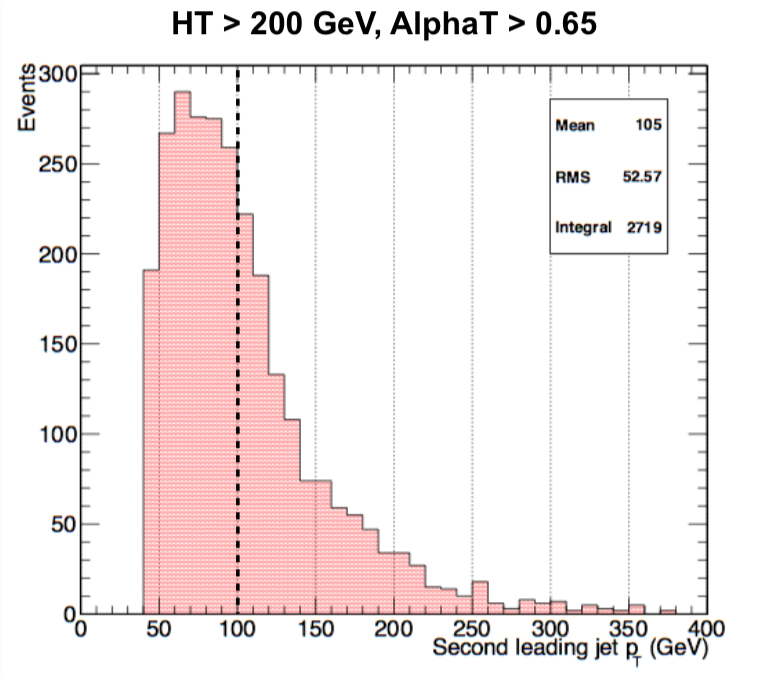
\includegraphics[width=0.5\textwidth]{figures/asymPlots/secondJetPtlowHT}
  }~~
  \subfigure[Second jet \PT for $400\gev<\HT>500\gev$, $\alphat>0.52$]{
    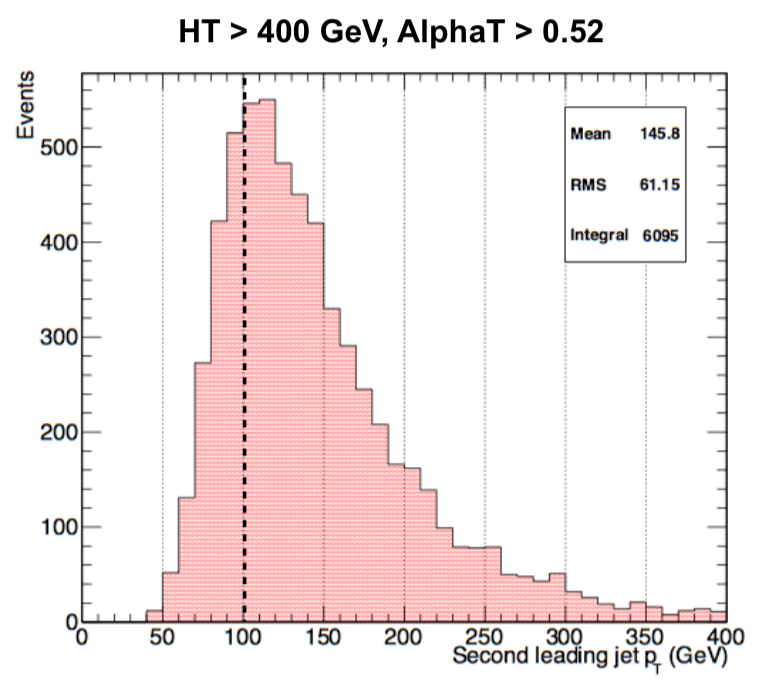
\includegraphics[width=0.5\textwidth]{figures/asymPlots/secondJetPthigherHT}
  }
  \\
  \caption{\label{fig:asymMotivation} The second leading jet \PT for different
  cases of \HT after a baseline signal selection: $\njet\geq2$, lead jet
  $\ET>100\gev$, lepton vetoes. Made with the T2tt ($m_{\rm
    stop}=425\gev$, $m_{\rm LSP}=325\gev$) simplified model sample.}
\end{figure}

